\subsection{Free Running Oscillator}
After completing a full capacitance test, the recorded data was graphed, as
shown in Figure~\ref{fig:free_run_c}.
%
\begin{figure}[H]
	\centering
	\begin{tikzpicture}[gnuplot]
%% generated with GNUPLOT 4.4p2 (Lua 5.1.4; terminal rev. 97, script rev. 96a)
%% Thu 17 Nov 2011 11:24:14 PM EST
\gpsolidlines
\gpcolor{gp lt color axes}
\gpsetlinetype{gp lt axes}
\gpsetlinewidth{1.00}
\draw[gp path] (1.688,0.985)--(9.014,0.985);
\gpcolor{gp lt color border}
\gpsetlinetype{gp lt border}
\draw[gp path] (1.688,0.985)--(1.868,0.985);
\node[gp node right] at (1.504,0.985) { 0.1};
\draw[gp path] (1.688,1.271)--(1.778,1.271);
\draw[gp path] (1.688,1.439)--(1.778,1.439);
\draw[gp path] (1.688,1.558)--(1.778,1.558);
\draw[gp path] (1.688,1.650)--(1.778,1.650);
\draw[gp path] (1.688,1.725)--(1.778,1.725);
\draw[gp path] (1.688,1.789)--(1.778,1.789);
\draw[gp path] (1.688,1.844)--(1.778,1.844);
\draw[gp path] (1.688,1.893)--(1.778,1.893);
\gpcolor{gp lt color axes}
\gpsetlinetype{gp lt axes}
\draw[gp path] (1.688,1.936)--(9.014,1.936);
\gpcolor{gp lt color border}
\gpsetlinetype{gp lt border}
\draw[gp path] (1.688,1.936)--(1.868,1.936);
\node[gp node right] at (1.504,1.936) { 1};
\draw[gp path] (1.688,2.223)--(1.778,2.223);
\draw[gp path] (1.688,2.390)--(1.778,2.390);
\draw[gp path] (1.688,2.509)--(1.778,2.509);
\draw[gp path] (1.688,2.601)--(1.778,2.601);
\draw[gp path] (1.688,2.676)--(1.778,2.676);
\draw[gp path] (1.688,2.740)--(1.778,2.740);
\draw[gp path] (1.688,2.795)--(1.778,2.795);
\draw[gp path] (1.688,2.844)--(1.778,2.844);
\gpcolor{gp lt color axes}
\gpsetlinetype{gp lt axes}
\draw[gp path] (1.688,2.888)--(5.522,2.888);
\draw[gp path] (8.830,2.888)--(9.014,2.888);
\gpcolor{gp lt color border}
\gpsetlinetype{gp lt border}
\draw[gp path] (1.688,2.888)--(1.868,2.888);
\node[gp node right] at (1.504,2.888) { 10};
\draw[gp path] (1.688,3.174)--(1.778,3.174);
\draw[gp path] (1.688,3.341)--(1.778,3.341);
\draw[gp path] (1.688,3.460)--(1.778,3.460);
\draw[gp path] (1.688,3.552)--(1.778,3.552);
\draw[gp path] (1.688,3.628)--(1.778,3.628);
\draw[gp path] (1.688,3.691)--(1.778,3.691);
\draw[gp path] (1.688,3.747)--(1.778,3.747);
\draw[gp path] (1.688,3.795)--(1.778,3.795);
\gpcolor{gp lt color axes}
\gpsetlinetype{gp lt axes}
\draw[gp path] (1.688,3.839)--(9.014,3.839);
\gpcolor{gp lt color border}
\gpsetlinetype{gp lt border}
\draw[gp path] (1.688,3.839)--(1.868,3.839);
\node[gp node right] at (1.504,3.839) { 100};
\draw[gp path] (1.688,4.125)--(1.778,4.125);
\draw[gp path] (1.688,4.293)--(1.778,4.293);
\draw[gp path] (1.688,4.411)--(1.778,4.411);
\draw[gp path] (1.688,4.504)--(1.778,4.504);
\draw[gp path] (1.688,4.579)--(1.778,4.579);
\draw[gp path] (1.688,4.643)--(1.778,4.643);
\draw[gp path] (1.688,4.698)--(1.778,4.698);
\draw[gp path] (1.688,4.746)--(1.778,4.746);
\gpcolor{gp lt color axes}
\gpsetlinetype{gp lt axes}
\draw[gp path] (1.688,4.790)--(9.014,4.790);
\gpcolor{gp lt color border}
\gpsetlinetype{gp lt border}
\draw[gp path] (1.688,4.790)--(1.868,4.790);
\node[gp node right] at (1.504,4.790) { 1000};
\gpcolor{gp lt color axes}
\gpsetlinetype{gp lt axes}
\draw[gp path] (1.688,0.985)--(1.688,4.790);
\gpcolor{gp lt color border}
\gpsetlinetype{gp lt border}
\draw[gp path] (1.688,0.985)--(1.688,1.165);
\node[gp node center] at (1.688,0.677) { 0.0001};
\draw[gp path] (2.157,0.985)--(2.157,1.075);
\draw[gp path] (2.778,0.985)--(2.778,1.075);
\draw[gp path] (3.096,0.985)--(3.096,1.075);
\gpcolor{gp lt color axes}
\gpsetlinetype{gp lt axes}
\draw[gp path] (3.247,0.985)--(3.247,4.790);
\gpcolor{gp lt color border}
\gpsetlinetype{gp lt border}
\draw[gp path] (3.247,0.985)--(3.247,1.165);
\node[gp node center] at (3.247,0.677) { 0.001};
\draw[gp path] (3.716,0.985)--(3.716,1.075);
\draw[gp path] (4.337,0.985)--(4.337,1.075);
\draw[gp path] (4.655,0.985)--(4.655,1.075);
\gpcolor{gp lt color axes}
\gpsetlinetype{gp lt axes}
\draw[gp path] (4.806,0.985)--(4.806,4.790);
\gpcolor{gp lt color border}
\gpsetlinetype{gp lt border}
\draw[gp path] (4.806,0.985)--(4.806,1.165);
\node[gp node center] at (4.806,0.677) { 0.01};
\draw[gp path] (5.275,0.985)--(5.275,1.075);
\draw[gp path] (5.896,0.985)--(5.896,1.075);
\draw[gp path] (6.214,0.985)--(6.214,1.075);
\gpcolor{gp lt color axes}
\gpsetlinetype{gp lt axes}
\draw[gp path] (6.365,0.985)--(6.365,2.425);
\draw[gp path] (6.365,3.349)--(6.365,4.790);
\gpcolor{gp lt color border}
\gpsetlinetype{gp lt border}
\draw[gp path] (6.365,0.985)--(6.365,1.165);
\node[gp node center] at (6.365,0.677) { 0.1};
\draw[gp path] (6.835,0.985)--(6.835,1.075);
\draw[gp path] (7.455,0.985)--(7.455,1.075);
\draw[gp path] (7.773,0.985)--(7.773,1.075);
\gpcolor{gp lt color axes}
\gpsetlinetype{gp lt axes}
\draw[gp path] (7.924,0.985)--(7.924,2.425);
\draw[gp path] (7.924,3.349)--(7.924,4.790);
\gpcolor{gp lt color border}
\gpsetlinetype{gp lt border}
\draw[gp path] (7.924,0.985)--(7.924,1.165);
\node[gp node center] at (7.924,0.677) { 1};
\draw[gp path] (8.394,0.985)--(8.394,1.075);
\draw[gp path] (9.014,0.985)--(9.014,1.075);
\draw[gp path] (9.014,0.985)--(8.834,0.985);
\node[gp node left] at (9.198,0.985) { 0};
\draw[gp path] (9.014,1.936)--(8.834,1.936);
\node[gp node left] at (9.198,1.936) { 15};
\draw[gp path] (9.014,2.888)--(8.834,2.888);
\node[gp node left] at (9.198,2.888) { 30};
\draw[gp path] (9.014,3.839)--(8.834,3.839);
\node[gp node left] at (9.198,3.839) { 45};
\draw[gp path] (9.014,4.790)--(8.834,4.790);
\node[gp node left] at (9.198,4.790) { 60};
\draw[gp path] (1.688,4.790)--(1.688,0.985)--(9.014,0.985)--(9.014,4.790)--cycle;
\node[gp node center,rotate=-270] at (0.246,2.887) {Output Frequency, $f$ (\si{\kilo\hertz})};
\node[gp node center,rotate=-270] at (10.087,2.887) {Output Duty Cycle, (\si{\percent})};
\node[gp node center] at (5.351,0.215) {Capacitance, $C_T$ (\si{\micro\farad})};
\node[gp node center] at (5.351,5.252) {Free-running Oscillator: Varying Capacitor};
\draw[gp path] (5.522,2.425)--(5.522,3.349)--(8.830,3.349)--(8.830,2.425)--cycle;
\draw[gp path] (5.522,3.349)--(8.830,3.349);
\node[gp node right] at (7.546,3.041) {$f$};
\gpcolor{gp lt color 0}
\gpsetlinetype{gp lt plot 0}
\gpsetlinewidth{3.00}
\draw[gp path] (7.730,3.041)--(8.646,3.041);
\draw[gp path] (1.688,3.998)--(2.157,3.851)--(2.496,3.735)--(3.247,3.237)--(3.716,3.019)%
  --(4.055,2.919)--(4.806,2.402)--(5.340,2.128)--(5.615,1.974)--(6.365,1.492)--(6.899,1.182)%
  --(7.174,1.032)--(7.924,1.494)--(8.458,1.169)--(8.733,1.021);
\gpsetpointsize{4.00}
\gppoint{gp mark 8}{(1.688,3.998)}
\gppoint{gp mark 8}{(2.157,3.851)}
\gppoint{gp mark 8}{(2.496,3.735)}
\gppoint{gp mark 8}{(3.247,3.237)}
\gppoint{gp mark 8}{(3.716,3.019)}
\gppoint{gp mark 8}{(4.055,2.919)}
\gppoint{gp mark 8}{(4.806,2.402)}
\gppoint{gp mark 8}{(5.340,2.128)}
\gppoint{gp mark 8}{(5.615,1.974)}
\gppoint{gp mark 8}{(6.365,1.492)}
\gppoint{gp mark 8}{(6.899,1.182)}
\gppoint{gp mark 8}{(7.174,1.032)}
\gppoint{gp mark 8}{(7.924,1.494)}
\gppoint{gp mark 8}{(8.458,1.169)}
\gppoint{gp mark 8}{(8.733,1.021)}
\gppoint{gp mark 8}{(8.188,3.041)}
\gpcolor{gp lt color border}
\node[gp node right] at (7.546,2.733) {Duty Cycle};
\gpcolor{gp lt color 1}
\gpsetlinetype{gp lt plot 1}
\draw[gp path] (7.730,2.733)--(8.646,2.733);
\draw[gp path] (1.688,3.084)--(2.157,3.433)--(2.496,3.604)--(3.247,3.985)--(3.716,4.048)%
  --(4.055,4.073)--(4.806,4.149)--(5.340,4.143)--(5.615,4.149)--(6.365,4.156)--(6.899,4.149)%
  --(7.174,4.181)--(7.924,4.156)--(8.458,4.188)--(8.733,4.162);
\gppoint{gp mark 5}{(1.688,3.084)}
\gppoint{gp mark 5}{(2.157,3.433)}
\gppoint{gp mark 5}{(2.496,3.604)}
\gppoint{gp mark 5}{(3.247,3.985)}
\gppoint{gp mark 5}{(3.716,4.048)}
\gppoint{gp mark 5}{(4.055,4.073)}
\gppoint{gp mark 5}{(4.806,4.149)}
\gppoint{gp mark 5}{(5.340,4.143)}
\gppoint{gp mark 5}{(5.615,4.149)}
\gppoint{gp mark 5}{(6.365,4.156)}
\gppoint{gp mark 5}{(6.899,4.149)}
\gppoint{gp mark 5}{(7.174,4.181)}
\gppoint{gp mark 5}{(7.924,4.156)}
\gppoint{gp mark 5}{(8.458,4.188)}
\gppoint{gp mark 5}{(8.733,4.162)}
\gppoint{gp mark 5}{(8.188,2.733)}
\gpcolor{gp lt color border}
\gpsetlinetype{gp lt border}
\gpsetlinewidth{1.00}
\draw[gp path] (1.688,4.790)--(1.688,0.985)--(9.014,0.985)--(9.014,4.790)--cycle;
%% coordinates of the plot area
\gpdefrectangularnode{gp plot 1}{\pgfpoint{1.688cm}{0.985cm}}{\pgfpoint{9.014cm}{4.790cm}}
\end{tikzpicture}
%% gnuplot variables

	\parbox{.6\textwidth}{
	\caption[Free Running Oscillator --- Varying $C_T$]{Recorded data for the
	varying capacitance test for a free running oscillator.  Note that the duty
	cycle remains reasonably constant above~\SI{0.01}{\micro\farad}, while the
	frequency decreases continuously.}
	\label{fig:free_run_c}}
\end{figure}
%
As is shown, the measured output frequency decreases linearly as the
capacitance increases (when plotted on a logarithmic scale), at a rate of
approximately~\SI{44.5}{\kilo\hertz\per\micro\farad}.  This is in line with the
expected behavior dictated by~\eqref{eq:t0_even}.  Similarly, the output's duty
cycle remains roughly constant for values over~\SI{0.01}{\micro\farad}, varying
at a rate of just~\SI{0.06}{\percent\per\micro\farad}.  Figure~\ref{fig:shot1}
shows the output signal for both a square wave and a triangular wave where the
value of~$C_T$ is~\SI{0.01}{\micro\farad}.
%
\begin{figure}[H]
	\centering
	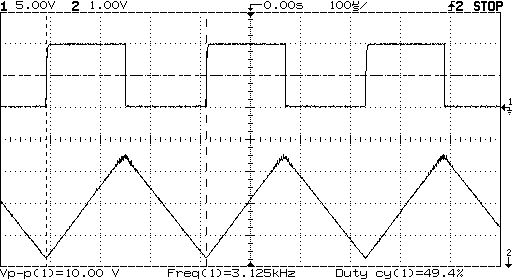
\includegraphics[width=.6\textwidth]{img/shot/shot1.png}
	\parbox{.6\textwidth}{
	\caption[Free Running Oscillator --- Varying~$C_T$ at~\SI{49.9}{\percent}
	Duty Cycle]{Oscilloscope capture of the triangular and square wave outputs
	of the VCO for a capacitance of~\SI{0.01}{\micro\farad}.  Note that the
	maximums of the triangular wave are synchronized with the rising edge of
	the square wave, implying an equal frequency for each.}
	\label{fig:shot1}}
\end{figure}
%
It is significant to note that the triangular wave has the same period as the
square wave in this screenshot, and that this will occur for all configurations
of the VCO.  As such, the triangular wave is omitted from all future
screenshots, as instructed by the course director.  While this configuration is
not an ideal~\SI{50}{\percent} duty cycle, it occurs at the capacitance above which
the duty cycle changes very little.  Additionally, said capacitance is one
element below the median value of the tested data set.

Similarly, the results of a varied resistance~$R_A$ can be seen in
Figure~\ref{fig:free_run_r}, below.
%
\begin{figure}[H]
	\centering
	\begin{tikzpicture}[gnuplot]
%% generated with GNUPLOT 4.4p2 (Lua 5.1.4; terminal rev. 97, script rev. 96a)
%% Thu 17 Nov 2011 08:55:20 PM EST
\gpsolidlines
\gpcolor{gp lt color axes}
\gpsetlinetype{gp lt axes}
\gpsetlinewidth{1.00}
\draw[gp path] (1.320,0.985)--(9.014,0.985);
\gpcolor{gp lt color border}
\gpsetlinetype{gp lt border}
\draw[gp path] (1.320,0.985)--(1.500,0.985);
\node[gp node right] at (1.136,0.985) { 0};
\gpcolor{gp lt color axes}
\gpsetlinetype{gp lt axes}
\draw[gp path] (1.320,1.461)--(9.014,1.461);
\gpcolor{gp lt color border}
\gpsetlinetype{gp lt border}
\draw[gp path] (1.320,1.461)--(1.500,1.461);
\node[gp node right] at (1.136,1.461) { 2};
\gpcolor{gp lt color axes}
\gpsetlinetype{gp lt axes}
\draw[gp path] (1.320,1.936)--(9.014,1.936);
\gpcolor{gp lt color border}
\gpsetlinetype{gp lt border}
\draw[gp path] (1.320,1.936)--(1.500,1.936);
\node[gp node right] at (1.136,1.936) { 4};
\gpcolor{gp lt color axes}
\gpsetlinetype{gp lt axes}
\draw[gp path] (1.320,2.412)--(9.014,2.412);
\gpcolor{gp lt color border}
\gpsetlinetype{gp lt border}
\draw[gp path] (1.320,2.412)--(1.500,2.412);
\node[gp node right] at (1.136,2.412) { 6};
\gpcolor{gp lt color axes}
\gpsetlinetype{gp lt axes}
\draw[gp path] (1.320,2.888)--(9.014,2.888);
\gpcolor{gp lt color border}
\gpsetlinetype{gp lt border}
\draw[gp path] (1.320,2.888)--(1.500,2.888);
\node[gp node right] at (1.136,2.888) { 8};
\gpcolor{gp lt color axes}
\gpsetlinetype{gp lt axes}
\draw[gp path] (1.320,3.363)--(9.014,3.363);
\gpcolor{gp lt color border}
\gpsetlinetype{gp lt border}
\draw[gp path] (1.320,3.363)--(1.500,3.363);
\node[gp node right] at (1.136,3.363) { 10};
\gpcolor{gp lt color axes}
\gpsetlinetype{gp lt axes}
\draw[gp path] (1.320,3.839)--(1.504,3.839);
\draw[gp path] (4.812,3.839)--(9.014,3.839);
\gpcolor{gp lt color border}
\gpsetlinetype{gp lt border}
\draw[gp path] (1.320,3.839)--(1.500,3.839);
\node[gp node right] at (1.136,3.839) { 12};
\gpcolor{gp lt color axes}
\gpsetlinetype{gp lt axes}
\draw[gp path] (1.320,4.314)--(1.504,4.314);
\draw[gp path] (4.812,4.314)--(9.014,4.314);
\gpcolor{gp lt color border}
\gpsetlinetype{gp lt border}
\draw[gp path] (1.320,4.314)--(1.500,4.314);
\node[gp node right] at (1.136,4.314) { 14};
\gpcolor{gp lt color axes}
\gpsetlinetype{gp lt axes}
\draw[gp path] (1.320,4.790)--(9.014,4.790);
\gpcolor{gp lt color border}
\gpsetlinetype{gp lt border}
\draw[gp path] (1.320,4.790)--(1.500,4.790);
\node[gp node right] at (1.136,4.790) { 16};
\gpcolor{gp lt color axes}
\gpsetlinetype{gp lt axes}
\draw[gp path] (1.320,0.985)--(1.320,4.790);
\gpcolor{gp lt color border}
\gpsetlinetype{gp lt border}
\draw[gp path] (1.320,0.985)--(1.320,1.165);
\node[gp node center] at (1.320,0.677) { 0};
\gpcolor{gp lt color axes}
\gpsetlinetype{gp lt axes}
\draw[gp path] (2.089,0.985)--(2.089,3.686);
\draw[gp path] (2.089,4.610)--(2.089,4.790);
\gpcolor{gp lt color border}
\gpsetlinetype{gp lt border}
\draw[gp path] (2.089,0.985)--(2.089,1.165);
\node[gp node center] at (2.089,0.677) { 2};
\gpcolor{gp lt color axes}
\gpsetlinetype{gp lt axes}
\draw[gp path] (2.859,0.985)--(2.859,3.686);
\draw[gp path] (2.859,4.610)--(2.859,4.790);
\gpcolor{gp lt color border}
\gpsetlinetype{gp lt border}
\draw[gp path] (2.859,0.985)--(2.859,1.165);
\node[gp node center] at (2.859,0.677) { 4};
\gpcolor{gp lt color axes}
\gpsetlinetype{gp lt axes}
\draw[gp path] (3.628,0.985)--(3.628,3.686);
\draw[gp path] (3.628,4.610)--(3.628,4.790);
\gpcolor{gp lt color border}
\gpsetlinetype{gp lt border}
\draw[gp path] (3.628,0.985)--(3.628,1.165);
\node[gp node center] at (3.628,0.677) { 6};
\gpcolor{gp lt color axes}
\gpsetlinetype{gp lt axes}
\draw[gp path] (4.398,0.985)--(4.398,3.686);
\draw[gp path] (4.398,4.610)--(4.398,4.790);
\gpcolor{gp lt color border}
\gpsetlinetype{gp lt border}
\draw[gp path] (4.398,0.985)--(4.398,1.165);
\node[gp node center] at (4.398,0.677) { 8};
\gpcolor{gp lt color axes}
\gpsetlinetype{gp lt axes}
\draw[gp path] (5.167,0.985)--(5.167,4.790);
\gpcolor{gp lt color border}
\gpsetlinetype{gp lt border}
\draw[gp path] (5.167,0.985)--(5.167,1.165);
\node[gp node center] at (5.167,0.677) { 10};
\gpcolor{gp lt color axes}
\gpsetlinetype{gp lt axes}
\draw[gp path] (5.936,0.985)--(5.936,4.790);
\gpcolor{gp lt color border}
\gpsetlinetype{gp lt border}
\draw[gp path] (5.936,0.985)--(5.936,1.165);
\node[gp node center] at (5.936,0.677) { 12};
\gpcolor{gp lt color axes}
\gpsetlinetype{gp lt axes}
\draw[gp path] (6.706,0.985)--(6.706,4.790);
\gpcolor{gp lt color border}
\gpsetlinetype{gp lt border}
\draw[gp path] (6.706,0.985)--(6.706,1.165);
\node[gp node center] at (6.706,0.677) { 14};
\gpcolor{gp lt color axes}
\gpsetlinetype{gp lt axes}
\draw[gp path] (7.475,0.985)--(7.475,4.790);
\gpcolor{gp lt color border}
\gpsetlinetype{gp lt border}
\draw[gp path] (7.475,0.985)--(7.475,1.165);
\node[gp node center] at (7.475,0.677) { 16};
\gpcolor{gp lt color axes}
\gpsetlinetype{gp lt axes}
\draw[gp path] (8.245,0.985)--(8.245,4.790);
\gpcolor{gp lt color border}
\gpsetlinetype{gp lt border}
\draw[gp path] (8.245,0.985)--(8.245,1.165);
\node[gp node center] at (8.245,0.677) { 18};
\gpcolor{gp lt color axes}
\gpsetlinetype{gp lt axes}
\draw[gp path] (9.014,0.985)--(9.014,4.790);
\gpcolor{gp lt color border}
\gpsetlinetype{gp lt border}
\draw[gp path] (9.014,0.985)--(9.014,1.165);
\node[gp node center] at (9.014,0.677) { 20};
\draw[gp path] (9.014,0.985)--(8.834,0.985);
\node[gp node left] at (9.198,0.985) { 0};
\draw[gp path] (9.014,1.461)--(8.834,1.461);
\node[gp node left] at (9.198,1.461) { 10};
\draw[gp path] (9.014,1.936)--(8.834,1.936);
\node[gp node left] at (9.198,1.936) { 20};
\draw[gp path] (9.014,2.412)--(8.834,2.412);
\node[gp node left] at (9.198,2.412) { 30};
\draw[gp path] (9.014,2.888)--(8.834,2.888);
\node[gp node left] at (9.198,2.888) { 40};
\draw[gp path] (9.014,3.363)--(8.834,3.363);
\node[gp node left] at (9.198,3.363) { 50};
\draw[gp path] (9.014,3.839)--(8.834,3.839);
\node[gp node left] at (9.198,3.839) { 60};
\draw[gp path] (9.014,4.314)--(8.834,4.314);
\node[gp node left] at (9.198,4.314) { 70};
\draw[gp path] (9.014,4.790)--(8.834,4.790);
\node[gp node left] at (9.198,4.790) { 80};
\draw[gp path] (1.320,4.790)--(1.320,0.985)--(9.014,0.985)--(9.014,4.790)--cycle;
\node[gp node center,rotate=-270] at (0.246,2.887) {Output Frequency, $f$ (\si{\kilo\hertz})};
\node[gp node center,rotate=-270] at (10.087,2.887) {Output Duty Cycle, (\si{\percent})};
\node[gp node center] at (5.167,0.215) {Resistance, $R_A$ (\si{\kilo\ohm})};
\node[gp node center] at (5.167,5.252) {Free-running Oscillator: Varying Resistor};
\draw[gp path] (1.504,3.686)--(1.504,4.610)--(4.812,4.610)--(4.812,3.686)--cycle;
\draw[gp path] (1.504,4.610)--(4.812,4.610);
\node[gp node right] at (3.528,4.302) {$f$};
\gpcolor{gp lt color 0}
\gpsetlinetype{gp lt plot 0}
\gpsetlinewidth{3.00}
\draw[gp path] (3.712,4.302)--(4.628,4.302);
\draw[gp path] (3.628,2.405)--(4.398,3.382)--(5.167,3.534)--(5.936,3.449)--(6.706,3.311)%
  --(7.475,3.152)--(8.245,2.996)--(9.014,2.852);
\gpsetpointsize{4.00}
\gppoint{gp mark 8}{(3.628,2.405)}
\gppoint{gp mark 8}{(4.398,3.382)}
\gppoint{gp mark 8}{(5.167,3.534)}
\gppoint{gp mark 8}{(5.936,3.449)}
\gppoint{gp mark 8}{(6.706,3.311)}
\gppoint{gp mark 8}{(7.475,3.152)}
\gppoint{gp mark 8}{(8.245,2.996)}
\gppoint{gp mark 8}{(9.014,2.852)}
\gppoint{gp mark 8}{(4.170,4.302)}
\gpcolor{gp lt color border}
\node[gp node right] at (3.528,3.994) {Duty Cycle};
\gpcolor{gp lt color 1}
\gpsetlinetype{gp lt plot 1}
\draw[gp path] (3.712,3.994)--(4.628,3.994);
\draw[gp path] (3.628,1.746)--(4.398,2.721)--(5.167,3.325)--(5.936,3.729)--(6.706,4.015)%
  --(7.475,4.234)--(8.245,4.405)--(9.014,4.547);
\gppoint{gp mark 5}{(3.628,1.746)}
\gppoint{gp mark 5}{(4.398,2.721)}
\gppoint{gp mark 5}{(5.167,3.325)}
\gppoint{gp mark 5}{(5.936,3.729)}
\gppoint{gp mark 5}{(6.706,4.015)}
\gppoint{gp mark 5}{(7.475,4.234)}
\gppoint{gp mark 5}{(8.245,4.405)}
\gppoint{gp mark 5}{(9.014,4.547)}
\gppoint{gp mark 5}{(4.170,3.994)}
\gpcolor{gp lt color border}
\gpsetlinetype{gp lt border}
\gpsetlinewidth{1.00}
\draw[gp path] (1.320,4.790)--(1.320,0.985)--(9.014,0.985)--(9.014,4.790)--cycle;
%% coordinates of the plot area
\gpdefrectangularnode{gp plot 1}{\pgfpoint{1.320cm}{0.985cm}}{\pgfpoint{9.014cm}{4.790cm}}
\end{tikzpicture}
%% gnuplot variables

	\parbox{.6\textwidth}{
	\caption[Free Running Oscillator --- Varying $R_A$]{Measured data for a
	varied resistance, as measured by an in-lab oscilloscope.}
	\label{fig:free_run_r}}
\end{figure}
%
In a striking contrast to the varying capacitor, a varying resistor shows a
consistently varying duty cycle and frequency.  This is expected behavior,
however, as described by~\eqref{eq:t0}.  It is interesting to note here the
peak value of the output frequency~(\SI{10.72}{\kilo\hertz} occurred at a
resistance of~\SI{10}{\kilo\hertz}, as this is also where the duty cycle was
measured closest to~\SI{50}{\percent}, at~\SI{49.2}{\percent}.
As~\SI{10}{\kilo\ohm} is the value of~$R_A$ used in the varying-capacitance
case~(which produced a roughly fifty-percent duty cycle for more than half of
its test range), this intuitively makes sense.  The waveform at this point can
be seen in Figure~\ref{fig:shot4}.
%
\begin{figure}[H]
	\centering
	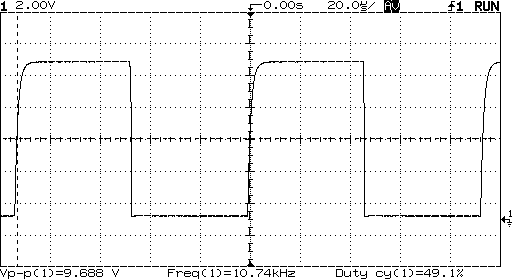
\includegraphics[width=.6\textwidth]{img/shot/shot4.png}
	\parbox{.6\textwidth}{
	\caption[Free Running Oscillator --- Varying $R_A$ at \SI{49.2}{\percent}
	Duty Cycle]{Screenshot of the free-running oscillator when the timing
	resistor $R_A$ is set at~\SI{10}{\kilo\ohm}}
	\label{fig:shot4}}
\end{figure}
%
As is expected, the frequency~(\SI{10.72}{\kilo\ohm} here
vs\.~\SI{10.97}{\kilo\ohm} previously) and duty cycle~(\SI{49.2}{\percent} here
vs\.~\SI{48.7}{\percent} previously) match closely the values recorded for the
system when~$C_T$ was varied, under roughly the same element values.  As an
extension of this test, students were asked to examine the fringe behavior of a
varying $R_A$ when it grows to be too large.  A maximum value
of~\SI{100}{\kilo\ohm} was used, and another oscilloscope screenshot was
captured.  It is shown here in Figure~\ref{fig:shot3}.
%
\begin{figure}[H]
	\centering
	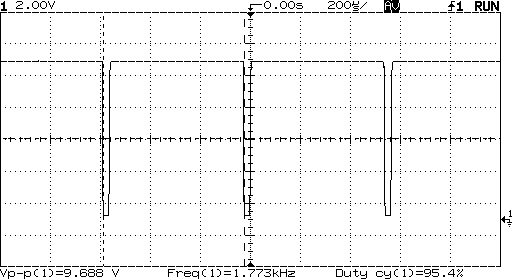
\includegraphics[width=.6\textwidth]{img/shot/shot3.png}
	\parbox{.6\textwidth}{
	\caption[Free Running Oscillator --- Varying $R_A$ at \SI{95.2}{\percent}
	Duty Cycle]{Edge-case behavior for a varying~$R_A$, showing a drastic
	change in duty cycle for a resistance change of just one order of
	magnitude.}
	\label{fig:shot3}}
\end{figure}
%
The captured oscilloscope data for the edge case of a varying timing resistor
shows that the data trends observed in Figure~\ref{fig:free_run_r} continue to
hold true for a much larger range of values.  What's more, this result shows
the importance of properly managing the value of the timing resistor.  If it
grows too large or, by extrapolation of the existing trends, too small, the
duty cycle of the output wave will extend toward~\SI{100}{\percent}
or~\SI{0}{\percent}, respectively.

\subsection{DC Sweep}
\begin{figure}[H]
	\centering
	Next, a DC sweep will be performed on the circuit to view the effects of input
voltage on the duty cycle.  This circuit will be based on the one shown in
Figure~\ref{fig:dc_sweep}.
%
\begin{figure}[H]
	\centering
	Next, a DC sweep will be performed on the circuit to view the effects of input
voltage on the duty cycle.  This circuit will be based on the one shown in
Figure~\ref{fig:dc_sweep}.
%
\begin{figure}[H]
	\centering
	Next, a DC sweep will be performed on the circuit to view the effects of input
voltage on the duty cycle.  This circuit will be based on the one shown in
Figure~\ref{fig:dc_sweep}.
%
\begin{figure}[H]
	\centering
	\input{schem/dc_sweep.tex}
	\caption{DC sweep schematic shown in Figure~5B of the Intersil ICL8038 datasheet [1].  All component values are the same as in Figure~\ref{fig:free_run}}
	\label{fig:dc_sweep}
\end{figure}
%
In this configuration, the negative lead of a DC voltage is connected to pin~8.
With all components as defined as in Figure~\ref{fig:dc_sweep}, the DC voltage
is varied from~\SI{1}{\volt} to~\SI{8}{\volt} in steps of
roughly~\SI{1}{\volt}.  When the input approaches eight volts, the output
quality will degrade.

\begin{figure}[H]
	\centering
	\input{img/plot/dc_sweep.tex}
\end{figure}

	\caption{DC sweep schematic shown in Figure~5B of the Intersil ICL8038 datasheet [1].  All component values are the same as in Figure~\ref{fig:free_run}}
	\label{fig:dc_sweep}
\end{figure}
%
In this configuration, the negative lead of a DC voltage is connected to pin~8.
With all components as defined as in Figure~\ref{fig:dc_sweep}, the DC voltage
is varied from~\SI{1}{\volt} to~\SI{8}{\volt} in steps of
roughly~\SI{1}{\volt}.  When the input approaches eight volts, the output
quality will degrade.

\begin{figure}[H]
	\centering
	Next, a DC sweep will be performed on the circuit to view the effects of input
voltage on the duty cycle.  This circuit will be based on the one shown in
Figure~\ref{fig:dc_sweep}.
%
\begin{figure}[H]
	\centering
	\input{schem/dc_sweep.tex}
	\caption{DC sweep schematic shown in Figure~5B of the Intersil ICL8038 datasheet [1].  All component values are the same as in Figure~\ref{fig:free_run}}
	\label{fig:dc_sweep}
\end{figure}
%
In this configuration, the negative lead of a DC voltage is connected to pin~8.
With all components as defined as in Figure~\ref{fig:dc_sweep}, the DC voltage
is varied from~\SI{1}{\volt} to~\SI{8}{\volt} in steps of
roughly~\SI{1}{\volt}.  When the input approaches eight volts, the output
quality will degrade.

\begin{figure}[H]
	\centering
	\input{img/plot/dc_sweep.tex}
\end{figure}

\end{figure}

	\caption{DC sweep schematic shown in Figure~5B of the Intersil ICL8038 datasheet [1].  All component values are the same as in Figure~\ref{fig:free_run}}
	\label{fig:dc_sweep}
\end{figure}
%
In this configuration, the negative lead of a DC voltage is connected to pin~8.
With all components as defined as in Figure~\ref{fig:dc_sweep}, the DC voltage
is varied from~\SI{1}{\volt} to~\SI{8}{\volt} in steps of
roughly~\SI{1}{\volt}.  When the input approaches eight volts, the output
quality will degrade.

\begin{figure}[H]
	\centering
	Next, a DC sweep will be performed on the circuit to view the effects of input
voltage on the duty cycle.  This circuit will be based on the one shown in
Figure~\ref{fig:dc_sweep}.
%
\begin{figure}[H]
	\centering
	Next, a DC sweep will be performed on the circuit to view the effects of input
voltage on the duty cycle.  This circuit will be based on the one shown in
Figure~\ref{fig:dc_sweep}.
%
\begin{figure}[H]
	\centering
	\input{schem/dc_sweep.tex}
	\caption{DC sweep schematic shown in Figure~5B of the Intersil ICL8038 datasheet [1].  All component values are the same as in Figure~\ref{fig:free_run}}
	\label{fig:dc_sweep}
\end{figure}
%
In this configuration, the negative lead of a DC voltage is connected to pin~8.
With all components as defined as in Figure~\ref{fig:dc_sweep}, the DC voltage
is varied from~\SI{1}{\volt} to~\SI{8}{\volt} in steps of
roughly~\SI{1}{\volt}.  When the input approaches eight volts, the output
quality will degrade.

\begin{figure}[H]
	\centering
	\input{img/plot/dc_sweep.tex}
\end{figure}

	\caption{DC sweep schematic shown in Figure~5B of the Intersil ICL8038 datasheet [1].  All component values are the same as in Figure~\ref{fig:free_run}}
	\label{fig:dc_sweep}
\end{figure}
%
In this configuration, the negative lead of a DC voltage is connected to pin~8.
With all components as defined as in Figure~\ref{fig:dc_sweep}, the DC voltage
is varied from~\SI{1}{\volt} to~\SI{8}{\volt} in steps of
roughly~\SI{1}{\volt}.  When the input approaches eight volts, the output
quality will degrade.

\begin{figure}[H]
	\centering
	Next, a DC sweep will be performed on the circuit to view the effects of input
voltage on the duty cycle.  This circuit will be based on the one shown in
Figure~\ref{fig:dc_sweep}.
%
\begin{figure}[H]
	\centering
	\input{schem/dc_sweep.tex}
	\caption{DC sweep schematic shown in Figure~5B of the Intersil ICL8038 datasheet [1].  All component values are the same as in Figure~\ref{fig:free_run}}
	\label{fig:dc_sweep}
\end{figure}
%
In this configuration, the negative lead of a DC voltage is connected to pin~8.
With all components as defined as in Figure~\ref{fig:dc_sweep}, the DC voltage
is varied from~\SI{1}{\volt} to~\SI{8}{\volt} in steps of
roughly~\SI{1}{\volt}.  When the input approaches eight volts, the output
quality will degrade.

\begin{figure}[H]
	\centering
	\input{img/plot/dc_sweep.tex}
\end{figure}

\end{figure}

\end{figure}

\end{figure}

\subsection{Frequency Modulation}
\begin{figure}[H]
	\centering
	\begin{circuitikz}
	\draw[ultra thick] (-2, -1.5) rectangle (2, 1.5);
	\draw[/tikz/circuitikz/bipoles/length=1cm]
	(-1.5, 1.5) node[below] {4} to [R, l=\SI{10}{\kilo\ohm}] ++(0, 1.5)
		to [short, -o] (4, 3) node[right] {$V+$}
	(0, 1.5) node[below] {5} to [R, l=\SI{+10}{\kilo\ohm}] ++(0, 1.5)
	(1.5, 1.5) node[below] {6} to [short] ++(0, 1.5)
	(3, 3) to [R, l_=\SI{10}{\kilo\ohm}] ++(0, -1.5) to [short] ++(0, -.5)

	(1.5, -1.5) node[above] {12} to [R, l=\SI{82}{\kilo\ohm}] ++(0, -1.5)
	(0, -1.5) node[above] {11} to [short] ++(0, -1.5)
	(-1.5, -1.5) node[above] {10} to [C, l=\SI{3.3}{\micro\farad}] ++(0, -1.5)
		to [short, -o] (4, -3) node[right] {$V-$};



%	(-2, 0) node[right] {8} to [short] ++(-.5, 0)
%		to [short] ++(0, 1) to [short] ++(.5, 0) node[right] {7};

	% short stuff on the right side
	\draw[/tikz/circuitikz/bipoles/length=.75cm]
	(2, 1) node[left] {9} to [short, -o] ++(2, 0)
	(2, .5) node[left] {3} to [short, -o] ++(2, 0)
		(3, .5) to [R, l=$R_\text{TRI}$] ++(0, -1) node[ground] {}
	(2, -1) node[left] {2} to [short, -o] ++(2, 0)
		(3, -1) to [R, l=$R_\text{SINE}$] ++(0, -1) node[ground] {}

	% short stuff on the left side
	(-2, 1) node[right] {7} to [short] ++(-0.5, 0)
		to [R, l_=\SI{10}{\kilo\ohm}] ++(0, -1) to [C, l_=\SI{10}{\micro\farad}, -o] ++(0, -.75) node[below] {FM}
	(-2, 0) node[right] {8} to [short] ++(-.5, 0);

	% square wave
	\draw[thick]
	(4.2, .85) -- ++(.1, 0) -- ++(0, .3)
		-- ++(.2, 0) -- ++(0, -.3) -- ++(.2, 0) -- ++(0, .3)
		-- ++(.2, 0) -- ++(0, -.3) -- ++(.1, 0);

	% triangle
	\draw[thick]
	(4.2, .5) -- ++(.1, .15) -- ++(.2, -.3) -- ++(.2, .3) -- ++(.2, -.3) --  ++(.1, .15);

	% sinusoid
	\draw[thick]
	(4.2, -1) sin ++(.1, .15) cos ++(.1, -.15) sin ++(.1, -.15) cos ++(.1, .15)
		sin ++(.1, .15) cos ++(.1, -.15) sin ++(.1, -.15) cos ++(.1, .15);
\end{circuitikz}

\end{figure}
